\section{实验预习}
\subsection{动态内存分配器的基本原理(5分)}
分配器将堆视为一组大小不同的块的集合来维护。每个块就是一个连续的虚拟内存片,要么是已经分配的,要么是空闲的,已分配的块显式地保留供应用程序使用。空闲块可用来分配。空闲块保持空闲,直到它显式地被应用程序所分配。一个已分配的块要么保持已分配状态,直到它被释放,这种释放要么是应用程序显式执行的,要么是内存分配器自身隐式执行的

\subsection{带边界标签的隐式空闲链表分配器原理(5分)}

\begin{figure}[H]
    \begin{minipage}[l]{0.6\linewidth}
        \heiti
        \begin{tikzpicture}
        \draw (0,0) rectangle +(8,8);
        \draw (7,7) -- (7,8);
        \draw (7,0) -- (7,1);
        \draw (0,1) -- (8,1);
        \draw (0,7) -- (8,7);
        \draw (0,3) -- (8,3);
        \draw (4,5) node{有效载荷};
        \draw (4,2) node{填充(可选)};
        \draw (3.5,0.5) node{块大小};
        \draw (3.5,7.5) node{块大小};
        \draw (7.5,0.5) node{a/f};
        \draw (7.5,7.5) node{a/f};
        \end{tikzpicture}
    \end{minipage}
    \begin{minipage}[c]{0.4\linewidth}
        \heiti
        空闲块通过头部的大小字段隐含的连接着,分配器通过遍历堆中所有的块,从而间接的遍历整个空闲块的集合。
        如果找不到合适的内存块,就对堆的大小进行扩展,需要注意的就是对空闲块的合并,使用了边界标记可以是使得这个操作变得很容易。
    \end{minipage}
\end{figure}


\subsection{显式空间链表的基本原理(5分)}
在内存块未被分配的时候,我们可以空闲的部分组织成显式的数据结构(比如双向链表),将数据结构存放在空闲块内部,在每个空闲块中都包含一个pred(前驱)和succ(后继)指针,正如下面右图所示。这样一来,就使得适配时间变成了空闲块数目的线性时间。
\begin{figure}[H]
    \begin{minipage}[c]{0.5\linewidth}
        \heiti
        \begin{tikzpicture}
        \draw (0,0) rectangle +(8,8);
        \draw (7,7) -- (7,8);
        \draw (7,0) -- (7,1);
        \draw (0,1) -- (8,1);
        \draw (0,7) -- (8,7);
        \draw (0,3) -- (8,3);
        \draw (4,5) node{有效载荷};
        \draw (4,2) node{填充(可选)};
        \draw (3.5,0.5) node{块大小};
        \draw (3.5,7.5) node{块大小};
        \draw (7.5,0.5) node{a/f};
        \draw (7.5,7.5) node{a/f};
        \end{tikzpicture}
        \caption{已分配}
    \end{minipage}
    \begin{minipage}[c]{0.5\linewidth}
        \heiti
        \begin{tikzpicture}
        \draw (0,0) rectangle +(8,8);
        \draw (7,7) -- (7,8);
        \draw (7,0) -- (7,1);
        \draw (0,1) -- (8,1);
        \draw (0,3) -- (8,3);
        \draw (0,5) -- (8,5);
        \draw (0,6) -- (8,6);
        \draw (0,7) -- (8,7);
        \draw (4,4) node{部分原载荷};
        \draw (4,2) node{填充(可选)};
        \draw (4,6.5) node{pred(祖先)};
        \draw (4,5.5) node{succ(后继)};
        \draw (3.5,0.5) node{块大小};
        \draw (3.5,7.5) node{块大小};
        \draw (7.5,0.5) node{a/f};
        \draw (7.5,7.5) node{a/f};
        \end{tikzpicture}
        \caption{未分配}
        
    \end{minipage}
\end{figure}

\subsection{红黑树的结构、查找、更新算法(5分)}
红黑树是每个节点都带有颜色属性的二叉查找树,颜色为红色或黑色。在二叉查找树强制一般要求以外,对于任何有效的红黑树我们增加了如下的额外要求使得红黑树相对平衡,从而保证了红黑树的查找、插入、删除的时间复杂度最坏为$O(log{n})$。

\begin{enumerate}
    \item 节点是红色或黑色
    \item 根是黑色
    \item 所有叶子都是黑色(叶子是NIL节点)
    \item 每个红色节点必须有两个黑色的子节点(从每个叶子到根的所有路径上不能有两个连续的红色节点)
    \item 从任一节点到其每个叶子的所有简单路径都包含相同数目的黑色节点
\end{enumerate}

红黑树的结构如图\ref{fig:red-blacktreeexample}所示:
\begin{figure}[H]
    \centering
    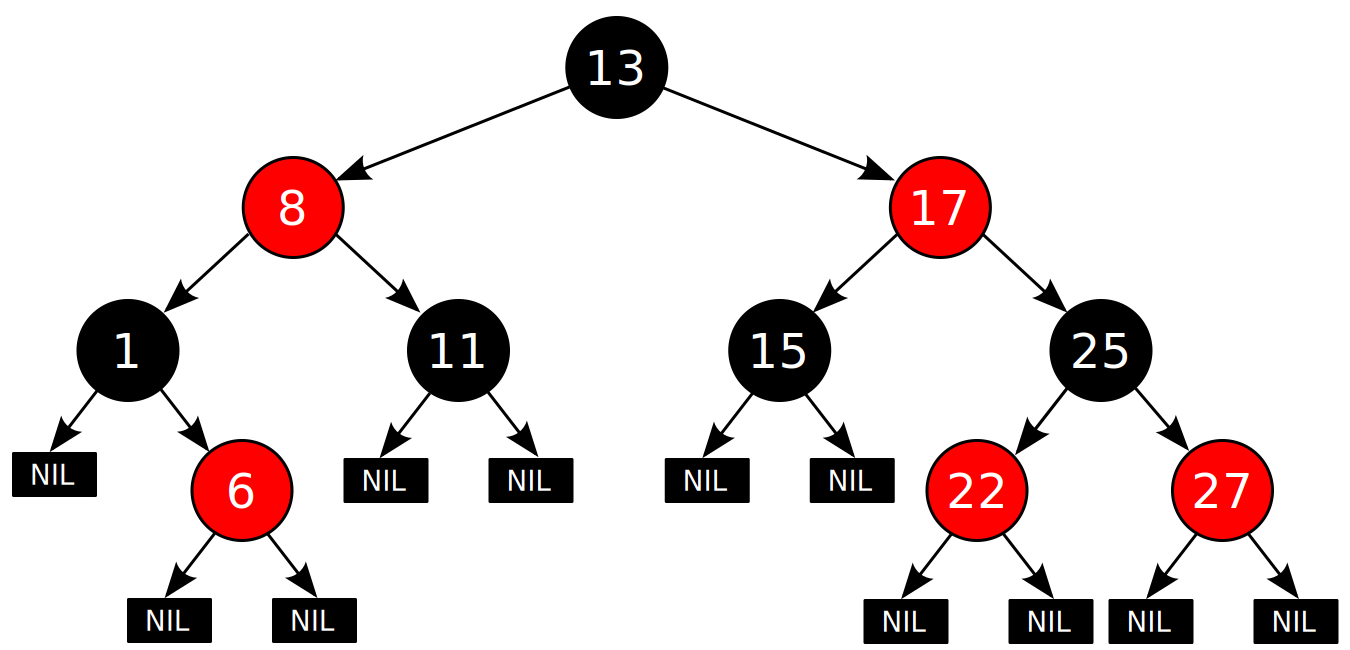
\includegraphics[width=0.7\linewidth]{figures/Red-black_tree_example}
    \caption{红黑树图例}
    \label{fig:red-blacktreeexample}
\end{figure}

查找算法非常简单,只需要进行递归的求解就可以了。更新分为插入和删除两种操作:

\textbf{插入:}
\begin{enumerate}
    \item 如果插入的是根结点,因为原树是空树,此情况只会违反性质2,所以直接把此结点涂为黑色。
    \item 如果插入的结点的父结点是黑色,由于此不会违反性质2和性质4,红黑树没有被破坏,所以此时也是什么也不做。
    \item 插入修复情况1:如果当前结点的父结点是红色且祖父结点的另一个子结点(叔叔结点)是红色
    \subitem 对策:将当前结点的父结点和叔叔结点涂黑,祖父结点涂红,把当前结点指向祖父结点,从新的当前结点重新开始算法。
    \item 插入修复情况2:当前结点的父结点是红色,叔叔结点是黑色,当前结点是其父结点的右子
    \subitem 对策:当前结点的父结点做为新的当前结点,以新当前结点为支点左旋。
    \item 插入修复情况3:当前结点的父结点是红色,叔叔结点是黑色,当前结点是其父结点的左子
    \subitem 对策:父结点变为黑色,祖父结点变为红色,在祖父结点为支点右旋
\end{enumerate}。

\textbf{删除:}
\begin{enumerate}
    \item 没有儿子,即为叶结点。直接把父结点的对应儿子指针设为NULL,删除儿子结点就OK了。
    \item 只有一个儿子。那么把父结点的相应儿子指针指向儿子的独生子,删除儿子结点也OK了。
    \item 有两个儿子。选择左儿子中的最大元素或者右儿子中的最小元素放到待删除结点的位置,保证结构的不变,而后调整子树。
\end{enumerate}

\begin{enumerate}
    \item 当前结点是红+黑色
    \subitem 对策:直接把当前结点染成黑色,结束此时红黑树性质全部恢复。
    \item 当前结点是黑+黑且是根结点
    \subitem 对策:什么都不做,结束。
    \item 删除修复情况1:当前结点是黑+黑且兄弟结点为红色(此时父结点和兄弟结点的子结点分为黑)
    \subitem 对策:把父结点染成红色,把兄弟结点染成黑色,之后重新进入算法
    \item 删除修复情况2:当前结点是黑加黑且兄弟是黑色且兄弟结点的两个子结点全为黑色
    \subitem 把当前结点和兄弟结点中抽取一重黑色追加到父结点上,把父结点当成新的当前结点,重新进入算法
    \item 删除修复情况3:当前结点颜色是黑+黑,兄弟结点是黑色,兄弟的左子是红色,右子是黑色
    \subitem 对策:把兄弟结点染红,兄弟左子结点染黑,之后再在兄弟结点为支点解右旋,之后重新进入算法
    \item 删除修复情况4:当前结点颜色是黑-黑色,它的兄弟结点是黑色,但是兄弟结点的右子是红色,兄弟结点左子的颜色任意
    \subitem 对策:把兄弟结点染成当前结点父结点的颜色,把当前结点父结点染成黑色,兄弟结点右子染成黑色,之后以当前结点的父结点为支点进行左旋,此时算法结束
\end{enumerate}




